%Texlive-full Version 3.141592-1.40.3 (Web2C 7.5.6)
%Kile Version 2.0.83
%File associated : SoFa_Logo.ps , FF.ps

\documentclass[a4paper,10pt]{article}
\usepackage[utf8x]{inputenc}
\usepackage[T1]{fontenc} 

\usepackage{lmodern}
\usepackage[a4paper]{geometry}
%\usepackage[frenchb]{babel}
\usepackage{graphicx}
\usepackage{hyperref}

\usepackage{pstricks}
\usepackage{pst-node}
%\usepackage{wrapfig}
\usepackage{amsmath}
\usepackage{amsfonts}
\usepackage{amssymb}
\usepackage{textcomp}
%\usepackage{mathaccent}

\usepackage{listings}
\lstset{language=C++,basicstyle=\scriptsize \color{green},identifierstyle=\color{orange},keywordstyle=[1]\color{blue},columns=fullflexible}

\usepackage{color}



\begin{document}
%%%%%%%%%%%%%%%%%%   LOGO  %%%%%%%%%%%%%%%%%%%%%%%%%
\begin{center}
\rput(6,1.5){\href{http://www.sofa-framework.org/}{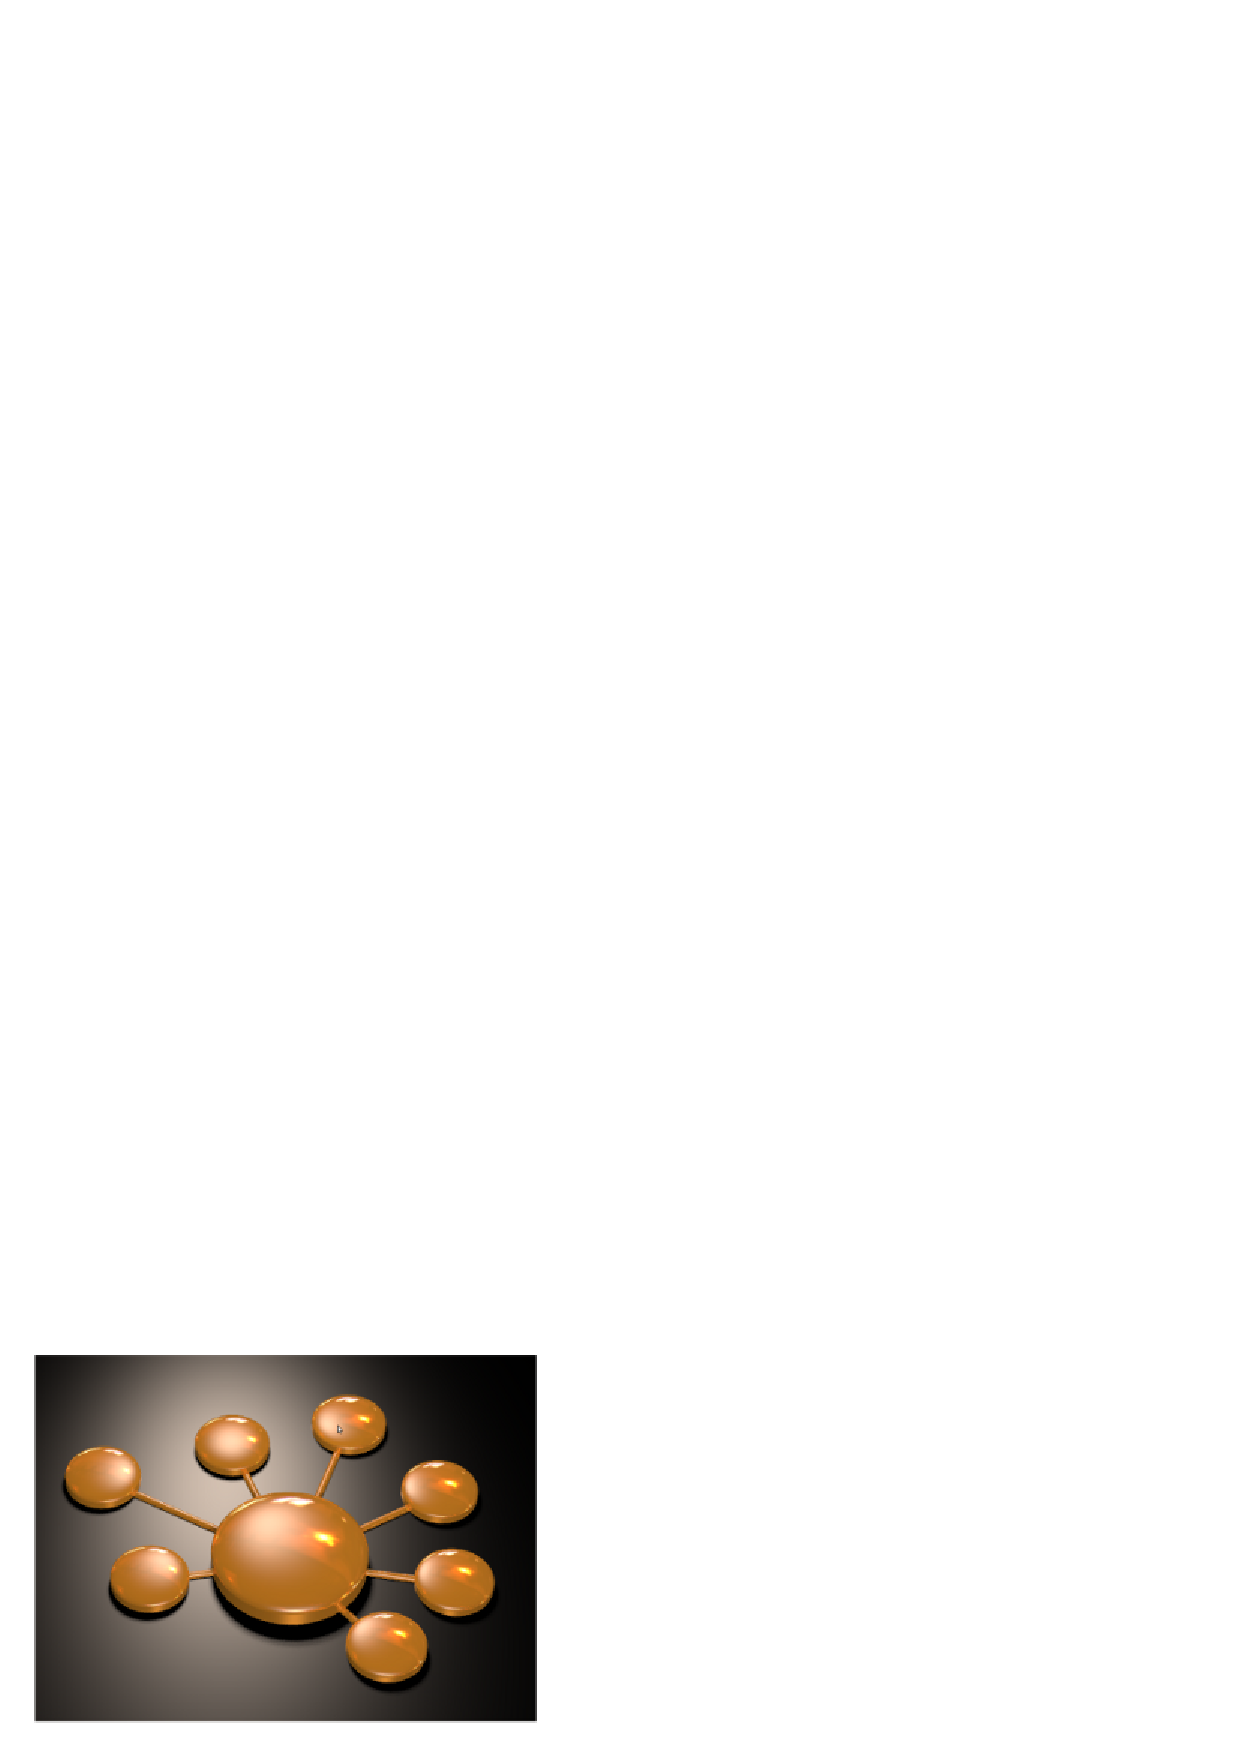
\includegraphics[scale=0.3]{SoFa_Logo}}}
\rput(-4,1.5){\href{http://www.sofa-framework.org/}{
		\begin{tabular}{l}
		\resizebox{4cm}{0.6cm}{SOFA} \\ 
		\resizebox{6cm}{0.3cm}{Simulation Open Framework Architecture}
		\end{tabular}
		}
	    }
\end{center}
%%%%%%%%%%%%%%%%%%   LOGO  %%%%%%%%%%%%%%%%%%%%%%%%%

%%%%%%%%%%%%%%%%%% DOCUMENT TITLE %%%%%%%%%%%%%%%%%%%%%%%%% To be deleted when include in the global document
%\chapter{Mapping} %\section{Rigid Mapping} 
\vspace{1.5cm}
\begin{center}\resizebox{7cm}{0.6cm}{FEM For Engeenering Material}\end{center}
%%%%%%%%%%%%%%%%%% DOCUMENT TITLE %%%%%%%%%%%%%%%%%%%%%%%%%

%%%%%%%%%%%%%%%%%%%%%%%%%%%%%%%%%%%%%%%%%%%%%%%%%%%%%%%%%%%%%%%%%%%%%%%%%%%%%%%%%%%%%%%%%
%=======================================================================================%
%%%%%%%%%%%%%%%%%%%%%%%%%%%%%%%%%%%%%%%%%%%%%%%%%%%%%%%%%%%%%%%%%%%%%%%%%%%%%%%%%%%%%%%%%
%\section{F.E.M}%%%%%%%%%%%%%%%%%%%%%%%

\section{FEM For Engeenering Material}

\paragraph{Abstract : }
Finite Element Method (FEM) is a technique for numerical resolving an partial differential equation (PDE). Several simplest examples of PDE can see as below : 
\begin{itemize}
 \item Heat Equation : \[ \frac{\partial u}{\partial t} - \alpha \bigtriangleup u = 0 \]
where $u : R^{3} \mapsto R $ is the temperature, the problem's solution.
 \item Stokes's problem :   \[ - \nu \bigtriangleup \textbf{v} + \bigtriangledown p = 0 \]
where $[\textbf{v},p] : R^{3} \mapsto R^{3}\bigotimes R $ is the velocity vector fields and the pressure, the problem's solution.
\end{itemize}
The finite element method aims at finding these solutions of the problem not in the continium form but the discrete one, approximated of the continium form. These functions, in the general form is a map from a domain to is codomain with respectively DIM\_DOMAIN and DIM\_CODOMAIN for dimensions. By this first-of-all functional definition, we can separate the notion of Element and Finite Element on the FEM configuration :
\begin{itemize}
 \item An Element Data Structure give locally all information on the domain of computation.
 \item An Finite Element Data Structure  give locally all information on its codomain. 
\end{itemize}    
   

\subsection{Equations for elastostatic: } 

\paragraph{Governing equations and Boundary problem: }
The set of equations on the boundery problem for elastostatic :
\[
\left\{
\begin{array}{rl}
 \text{div }\textbf{C.E} \left[ \textbf{u} \right] + \textbf{b} & =0 \\
                                       \textbf{u} & = \textbf{\^{u}} \text{         on $\partial\Omega_1 $}\\
           \textbf{C.E} \left[ \textbf{u} \right] &= \textbf{\^{s}}  \text{         on $\partial\Omega_2 $}
\end{array}\right.
\]
\paragraph{Variational formulation: }
Using the virtual displacement principe, this boundary problam is equivalent to a variational (weak) formulation problem :
\[
\left\{
\begin{array}{l}
\text {For every virtual displacement \textbf{u}$^*$ :} \\
  \int_{\Omega}\textbf{E}\left(\textbf{u}^*\right) ^t .\textbf{C[E} \left( \textbf{u} \right) \textbf{]} .dV
 -\int_{\Omega}\left[\textbf{u}^*\right]^t . \textbf{b} .dV
 -\int_{\partial\Omega_2}\left[\textbf{u}^* \right]^t \textbf{\^{s}.n} .dS  =0 \\
                                      
 \textbf{u} \text{ and } \textbf{u}^*\subset \text{ a appropriate functional space.}
\end{array}\right.
\]
Given a variational formulation in the integration formula, the aim of work in construction finite element is to be able to construct the stifness matrix :
\[
 K=\int_{\Omega}\textbf{E}\left(\textbf{u}^*\right) ^t .\textbf{C[E} \left( \textbf{u} \right) \textbf{]} .dV
\]
by filling in a double loop :
\[
\left\|
\begin{array}{l}
\text{for i=0 to nbDOFs} \\ 
\hspace{1cm} \text{for j=0 to nbDOFs} \\
\hspace{2cm} \text{K}_{ij} = \int_{\Omega} [...]^t .[...]dV  ;
\end{array}
\right.
\]

%\subsection{Equations for elastodynamic: }
%\paragraph{Governing equations and Boundary problem: }
%\paragraph{Variational formulation: }
\subsection{Coordinates definitions and notations: }
This section talks about different notions of coordinates in different view point. One can see that in the mathematical view, a reference element are usually defined by the unit canonical element, which may give ease for a generic finite element type : quadrature points, nodes on element, interpolation functions ... All elements differ only by their coordinate and not by its behavior. It's the reason that for all computation (interpolation, integration on quadrature), all elements are transformed to this reference element, after computing, the result may be taken by the revert of this transformation. This manner comes from the fact that for all elements, there exist an invertible affine transform to the reference element. By the mecanical view, the reference configuration reffer to the initial coordinate of the material (Lagrangian coordinates). It make difference from the current configuration of the material (Eulerian coordinates). These two different definitions of coordinates in continium mechanic make sens when using different descriptions (Eulerian, Lagrangian, or mixted) and by consequence differ the mechanical equations. Therefor, one define here for these different coordiantes. 
\begin{itemize}
 \item \textbf{Barycentric coordinates in the reference element: }These coordinates will be noted with a hat above the variables $\hat{\textbf{X}}$.
 \item \textbf{Lagrangian coordinates: }These reffer to the initial material coordinate without sollicitation \textbf{X}.
 \item \textbf{Eulerian coordinates: }These reffer to the curent coordinate (or spatial coordinate) when subitted a sollicitation textbf{x}.
\end{itemize}
\subsection{Coordinates transformation: }
\paragraph{Geometry affine mapping: }
Mathematically, for all elements, there exist a invertible affine transform that map a element to the reference element : $ \hat{\textbf{X}} = \textbf{T(X)} =\textbf{A.X} + \textbf{b}$ or in matrix notation :
\[
\left[
\begin{array}{c}
               \\
    \hat{X}_i  \\
               \\
\end{array}
\right]
=
\left[
\begin{array}{ccc}
  &                 & \\
  &  \text{A}_{ij}  & \\
  &                 & 
\end{array}
\right]
\left[
\begin{array}{c}
         \\
    X_j  \\
         \\     
\end{array}
\right]
+
\left[
\begin{array}{c}
         \\
    b_j  \\
         \\      
\end{array}
\right]
\]
Because this is a affine transform, one can see by the differential computing :
\[
\text{A}_{ij} = \frac{\partial \hat{X}_i }{\partial X_i} 
\]
This differential formule give the meanner for evaluating values and derivative values of interpolation functions. In general, a real interpolation functions can be defined in two variables $p(\hat{\textbf{X}}) = p(T^{-1}\textbf{(X)})$ . For evaluating the differential, whe can have the chain rule :   
\[
  \frac{\partial p}{\partial X_j}  = \frac{\partial p}{\partial \hat{X}_i } . \frac{\partial \hat{X}_i }{\partial X_j}
\]

\paragraph{Deformation gradient (Jacobian): }
Mechanically, for all admissible states, there exist a linear invertible transformation, which transform the initial material positions to the current material positions. This transformation are usually called Jacobian in the continium mechanic.
 \[
\begin{array}{ll}
\text{Motion equation                : } & \textbf{x}=\phi(\textbf{X},t) \\
\text{Deformation gradiant \textbf{F}: } & \textbf{F}=\frac{\partial \textbf{x}}{\partial \textbf{X}}  \text{   or d\textbf{x}=\textbf{F.} d\textbf{X} }
\end{array}
\]




\subsection{Interpolation: } 
To construct the stifness matrix, two components are needed to be defined in a generic elelemnt (master element): 
\begin{itemize}
\item Interpolation function (usually polynomial).\footnote{when talking about defining a function, that its values on any point, and eventually its derivative values at any point }
\item Quadrature formula (quadrature points and its weight). 
\end{itemize}
\paragraph{Several standard shape functions on tetrahedral element: }
\begin{center}
\begin{pspicture}(-7,-4)(7,4)
%\psline(-7,-2)(7,2)
\rput( 0  , 3.0){\Rnode{N0}{\color{blue}0}}
\rput(-3  ,-3  ){\Rnode{N1}{\color{blue}1}}
\rput( 6  ,-2.5){\Rnode{N2}{\color{blue}2}}
\rput( 0.0, 0.0){\Rnode{N3}{\color{blue}3}}

\rput(-1.5, 0.0 ){\Rnode{N01}{\color{blue}01}}
\rput( 3  , 0.25){\Rnode{N02}{\color{blue}02}}
\rput( 0.0, 1.5 ){\Rnode{N03}{\color{blue}03}}
\rput( 1.5,-2.75){\Rnode{N12}{\color{blue}12}}
\rput(-1.5,-1.5 ){\Rnode{N13}{\color{blue}13}}
\rput( 3.0,-1.25){\Rnode{N23}{\color{blue}23}}

\rput(0,-1.0){\Rnode{x}{\color{red} \textbullet}}
\rput(0,-1.0){\Rnode{P}{\color{red}PBull}}

\psline[showpoints=true](0,3.0)(-3,-3)(6,-2.5)(0,3.0)%N0N1N2N0
\psline[showpoints=true, linestyle=dashed](0,0)(0,3.0)%N3N0
\psline[showpoints=true, linestyle=dashed](0,0)(-3,-3)%N3N1
\psline[showpoints=true, linestyle=dashed](0,0)(6,-2.5)%N3N2
\end{pspicture}
\end{center}
\begin{itemize}
\item Lagrange P1
    \[
    \left\|
    \begin{array}{l}
    \text{for i=0 to nbVERTEX} \\ 
    \hspace{1cm} \omega^i = \lambda_i ;
    \end{array}
    \right.
    \]
\item Lagrange P1Bull
    \[
    \left\|
    \begin{array}{l}
    \text{for i=0 to nbVERTEX} \\ 
    \hspace{1cm} \omega^i = \lambda_i ; \\
    \omega^4 = \lambda_0 \lambda_1 \lambda_2 \lambda_3 ;
    \end{array}
    \right.
    \]
\item Lagrange P2
    \[
    \left\|
    \begin{array}{l}
    \text{for i=0 to nbVERTEX} \\ 
    \hspace{1cm} \omega^i = 2.\lambda_i^2 - \lambda_i ; \\
    \text{for j=0 to nbEDGE} \\
    \hspace{1cm}  i=j+\text{nbVERTEX};  \\
    \hspace{1cm}  [l;m]=\text{getLocalEdge(j)};  \\
    \hspace{1cm}  \omega^i = 4.\lambda_l \lambda_m ;
    \end{array}
    \right.
    \]
\end{itemize}


\paragraph{Several standard shape functions on hexahedral element: }
\begin{center}
\begin{pspicture}(-7,-4)(7,4)
%\psline(-7,-2)(7,2)
\rput(-5  , -4){\Rnode{N0}{\color{blue}0}}
\rput( 0  , -4){\Rnode{N1}{\color{blue}1}}
\rput( 2  , -2){\Rnode{N2}{\color{blue}2}}
\rput(-3  , -2){\Rnode{N3}{\color{blue}3}}

\rput(-5  ,  1){\Rnode{N4}{\color{blue}4}}
\rput( 0  ,  1){\Rnode{N5}{\color{blue}5}}
\rput( 2  ,  3){\Rnode{N6}{\color{blue}6}}
\rput(-3  ,  3){\Rnode{N7}{\color{blue}7}}

%\rput(-1.5, 0.0 ){\Rnode{N01}{\color{blue}01}}
%\rput( 3  , 0.25){\Rnode{N02}{\color{blue}02}}
%\rput( 0.0, 1.5 ){\Rnode{N03}{\color{blue}03}}
%\rput( 1.5,-2.75){\Rnode{N12}{\color{blue}12}}
%\rput(-1.5,-1.5 ){\Rnode{N13}{\color{blue}13}}
%\rput( 3.0,-1.25){\Rnode{N23}{\color{blue}23}}

%\rput(0,-1.0){\Rnode{x}{\color{red} \textbullet}}
%\rput(0,-1.0){\Rnode{P}{\color{red}PBull}}

\psline[showpoints=true](-5  , -4)( 0  , -4)( 0  ,  1)(-5  ,  1)(-5  , -4)%N0N1N5N4N0
\psline[showpoints=true](-5  ,  1)(-3  ,  3)( 2  ,  3)( 2  , -2)( 0  , -4)%N4N7N6N2N1
\psline[showpoints=true]( 0  ,  1)( 2  ,  3)%N5N6
\psline[showpoints=true, linestyle=dashed](-3  , -2)(-5  , -4)%N3N0
\psline[showpoints=true, linestyle=dashed](-3  , -2)( 2  , -2)%N3N2
\psline[showpoints=true, linestyle=dashed](-3  , -2)(-3  ,  3)%N3N7
\end{pspicture}
\end{center}
\begin{itemize}
%N_i= 1/8 (1 + x.x_i)(1 + y.y_i)(1 + z.z_i)
\item Lagrange P1
    \[
    \left\|
    \begin{array}{l}
    \text{for i=0 to nbVERTEX} \\ 
    \hspace{1cm} \omega^i = \frac{1}{8}. (1 + \xi_i .\xi)(1 + \eta_i .\eta)(1 +\mu_i .\mu ) ;
    \end{array}
    \right.
    \]
\item Lagrange P1Bull
    \[
    \left\|
    \begin{array}{l}
    \text{for i=0 to nbVERTEX} \\ 
    \hspace{1cm} \omega^i = \frac{1}{8}. (1 + \xi_i .\xi)(1 + \eta_i .\eta)(1 +\mu_i .\mu ) ; \\
    \omega^8 = (1 - \xi^2)(1 - \eta^2)(1 -\mu^2 ) ;
    \end{array}
    \right.
    \]
\item Lagrange Serendipity 20 Nodes
    \[
    \left\|
    \begin{array}{l}
    \text{for i=0 to nbVERTEX} \\ 
    \hspace{1cm} \omega^i = \frac{1}{8}. (1 + \xi_i .\xi)(1 + \eta_i .\eta)(1 +\mu_i .\mu )(\xi_i .\xi + \eta_i .\eta + \mu_i .\mu -2) ; \\
    \text{for j=0 to nbEDGE} \\
    \hspace{1cm}  i=j+\text{nbVERTEX};  \\
    \hspace{1cm}  [l;m]=\text{getLocalEdge(j)};  \\
    \hspace{1cm}  \text{if edge parallel to } O\xi  : \frac{1}{4}.(1 - \xi^2)(1 + \eta_l .\eta)(1 +\mu_l .\mu ) ; \\
    \hspace{1cm}  \text{if edge parallel to } O\eta : \frac{1}{4}.(1 - \eta^2)(1 + \xi_l .\xi)((1 +\mu_l .\mu ) ; \\
    \hspace{1cm}  \text{if edge parallel to } O\mu  : \frac{1}{4}.(1 -\mu^2 )(1 + \xi_l .\xi)(1 + \eta_l .\eta) ; 
    \end{array}
    \right.
    \]
\item Lagrange P2
    \[
    \left\|
    \begin{array}{l}
    \text{for i=0 to nbVERTEX} \\ 
    \hspace{1cm} \omega^i = \frac{1}{8}. (\xi^2 + \xi_i .\xi)(\eta^2 + \eta_i .\eta)(\mu^2 +\mu_i .\mu ) ; \\
    \text{for j=0 to nbEDGE} \\
    \hspace{1cm}  i=j+\text{nbVERTEX};  \\
    \hspace{1cm}  [l;m]=\text{getLocalEdge(j)};  \\
    \hspace{1cm}  \text{if edge parallel to } O\xi  : \frac{1}{4}.(1 - \xi^2)(\eta^2 + \eta_l .\eta)(\mu^2 +\mu_l .\mu ) ; \\
    \hspace{1cm}  \text{if edge parallel to } O\eta : \frac{1}{4}.(1 - \eta^2)(\xi^2 + \xi_l .\xi)(\mu^2 +\mu_l .\mu ) ; \\
    \hspace{1cm}  \text{if edge parallel to } O\mu  : \frac{1}{4}.(1 -\mu^2 )(\xi^2 + \xi_l .\xi)(\eta^2 + \eta_l .\eta) ; \\
    \text{for k=0 to nbFACE} \\
    \hspace{1cm}  i=k+\text{nbVERTEX+nbFACE};  \\
    \hspace{1cm}  [a;b;c;d]=\text{getLocalQuad(k)};  \\
    \hspace{1cm}  \text{if face perpendicular to } O\xi  : \frac{1}{2}.(\xi^2 + \xi_a .\xi)   (1 - \eta^2)(1 -\mu^2 ) ; \\
    \hspace{1cm}  \text{if face perpendicular to } O\eta : \frac{1}{2}.(\eta^2 + \eta_a .\eta)(1 - \xi^2) (1 -\mu^2 ) ; \\
    \hspace{1cm}  \text{if face perpendicular to } O\mu  : \frac{1}{2}.(\mu^2 +\mu_a .\mu )   (1 - \xi^2)(1 - \eta^2) ; \\
    \omega^{26} = (1 - \xi^2)(1 - \eta^2)(1 -\mu^2 ) ;
    \end{array}
    \right.
    \]
\end{itemize}


In litterature of numerical integration, quadrature points are usually given by its barycentric coordinates on element, and its weight. The quadrature formula is simply a set of quadrature poins, allowing to compute for any function :
\[
\int_{\Omega} fdV \approx \sum_{i=0}^{nbQP} qp[i].weight*f(qp[i])
\]
where $qp[i]$ is the i-th quadrature point, $nbQP$ is the number of quadrature points. Thus, defining a quadrature formular is simply defining a set of quadrature points, with some operator allowing to convert barycentric coordinate to cartesian coordinate and invert. 
\begin{center}
 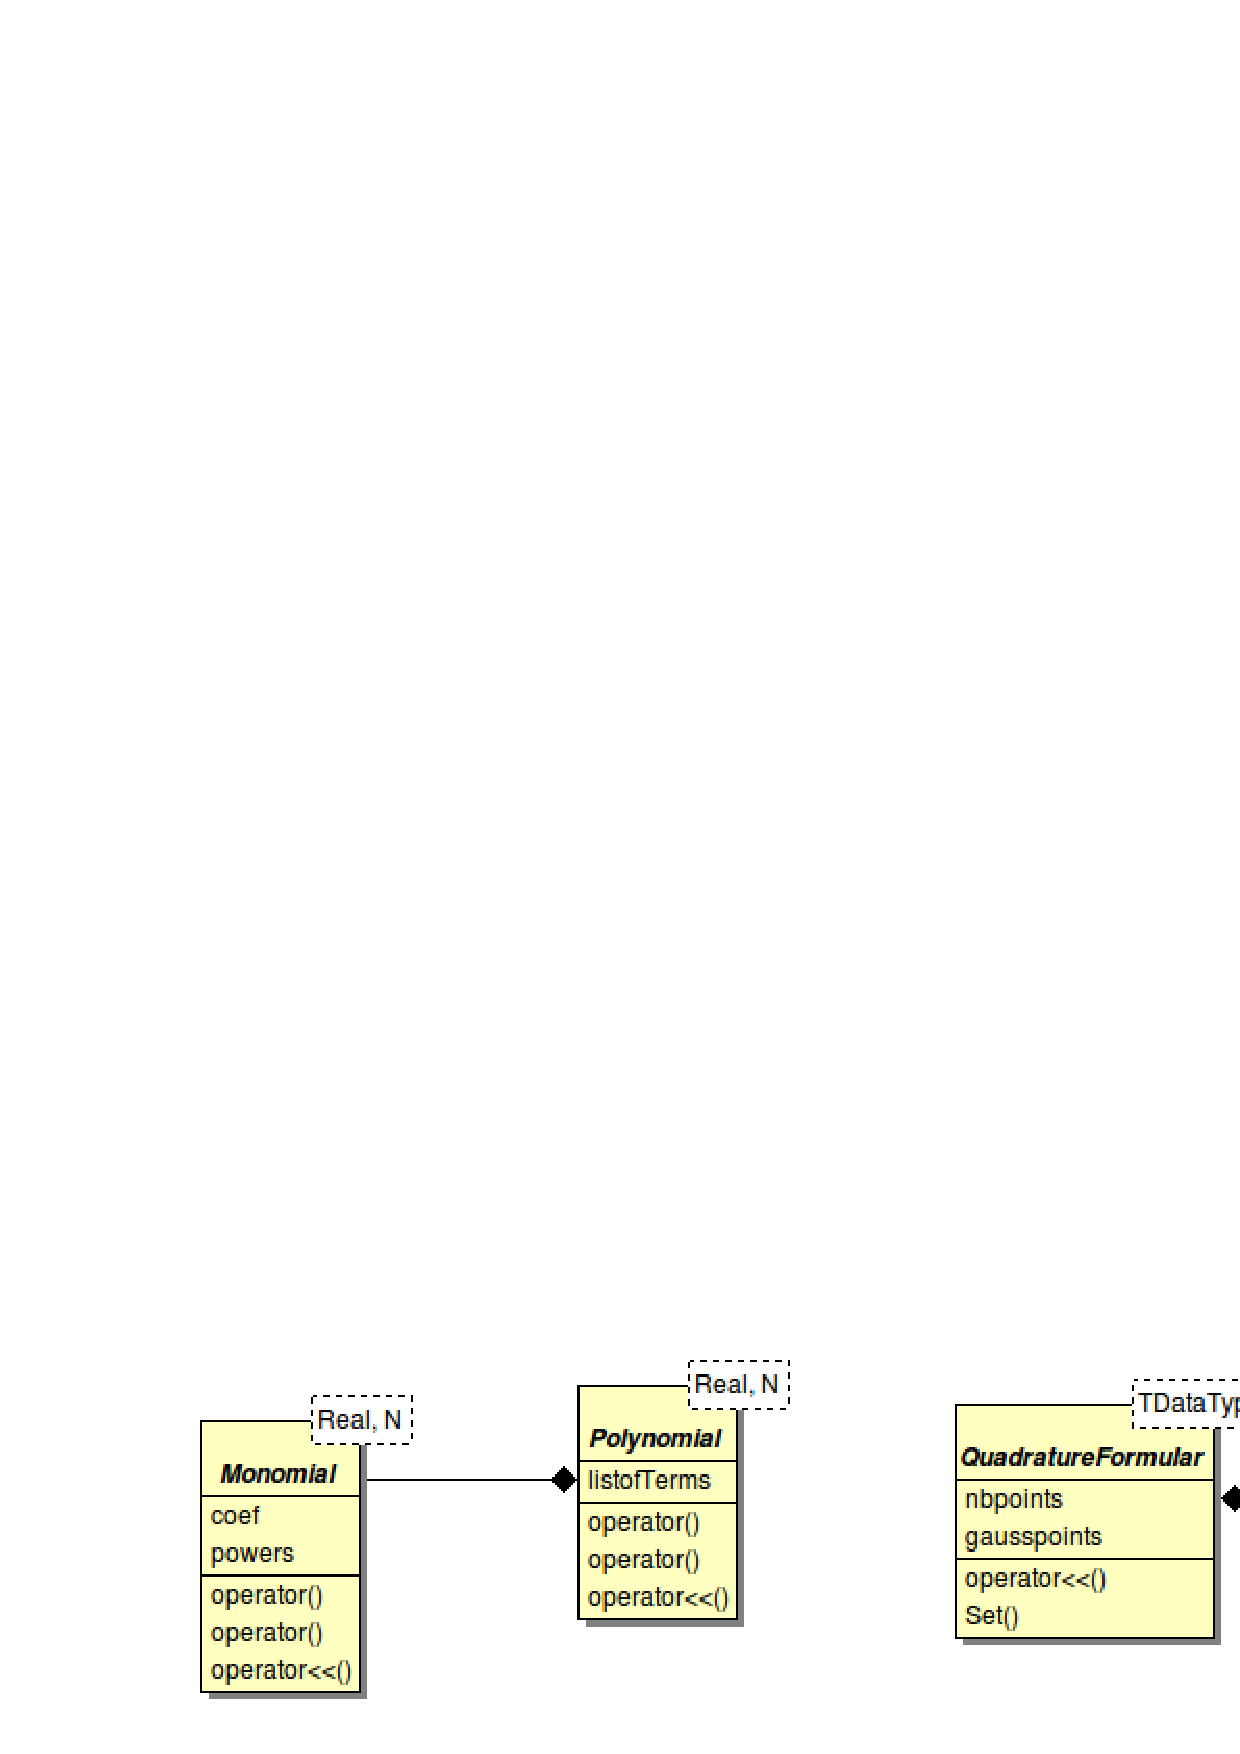
\includegraphics[scale=0.5]{diagramToolsFEM}
\end{center}

The same things for the polynomials : the polynomials are defined in the master element (generic), so in relation with the barycentric coordinate. There for, to evaluating its values and its derivate values on a point, sometime a change basis coordinate is needed, and a storage of this change of basis help to compute the gradian easily. For example in the dimension RdDIM = 3, interpolation polynomials are defined in RdDIM+1=4 variables \footnote{barycentric coordinates has one more variable than cartesian coordinates in the simplex geometry, but there are a linear transformation invertible make equivalent to these two presentations}. On a simplex element (tetrahedron), a polynomial is function of barycentric coordinate : 
\[
\phi_i =p_i(\lambda_0 , \lambda_1 , \lambda_2 , \lambda_3)
\]
Barycentric coordinate and cartesian coordinate are related by a linear transform unique invertible : 
\[
\begin{array}{cc}
\left[
\begin{array}{lll}
& & \\
& & \\
& & \\
& & 
\end{array}
\right]
\\
\left[F\right]
\end{array}
\\
\begin{array}{cc}
\\
\left[
\begin{array}{l}
x_0 \\
x_1 \\
x_2 
\end{array}
\right]
\\
X
\end{array}
=
\begin{array}{cc}
\left[
\begin{array}{lllll}
\lambda_0 \\
\lambda_1 \\
\lambda_2 \\
\lambda_3 
\end{array}
\right]
\\
\lambda
\end{array}
\]
\begin{center}
\begin{pspicture}(-7,-2)(7,2)
%\psline(-7,-2)(7,2)
\rput(0,1.7){\Rnode{A}{\color{blue}A}}
\rput(-1.2,-1.2){\Rnode{B}{\color{blue}B}}
\rput(4.2,-1.4){\Rnode{C}{\color{blue}C}}
\rput(0.2,0.2){\Rnode{D}{\color{blue}D}}

\rput(1,0){\Rnode{x}{\color{red} \textbullet}}
\rput(1,-0.5){\Rnode{P}{\color{red}P}}

\psline[showpoints=true](0,1.5)(-1,-1)(4,-1.4)(0,1.5)
\psline[showpoints=true, linestyle=dashed](0,0)(0,1.5)
\psline[showpoints=true, linestyle=dashed](0,0)(-1,-1)
\psline[showpoints=true, linestyle=dashed](0,0)(4,-1.4)
\end{pspicture}
\end{center}

To have this transformation, it is not needed to fill the matrix F, but the computing can be done by the geometry calculus. For a tetrahedron ABCD, and any point, P, how to compute its barycentric coordinate {$\lambda_A, \lambda_B, \lambda_C, \lambda_D $} relatively to the tetrahedron ABCD:
 \[
\lambda_A=\frac{ \text{volume }ABCD }{ \text{volume }PBCD } =\frac{\frac{1}{6} PC* (BC \wedge CD) }{\frac{1}{6} AC* (BC \wedge CD) }
\]
To be remarked this presentation in brief term : 
 \[
\lambda_A=\frac{{\color{red}\overrightarrow{PC}} * {\color{blue}(\overrightarrow{BC} \wedge \overrightarrow{CD})} }{ {\color{blue}\overrightarrow{AC}*(\overrightarrow{BC} \wedge \overrightarrow{CD})} }={\color{red}\overrightarrow{PC}}*{\color{blue}\overrightarrow{T}}  \text{ , T is a constant vector}
\]
There for, it is easily to compute gradian of $\lambda_A$ : 
 \[
\overrightarrow{Grad} \lambda_A=\color{blue} \overrightarrow{T} =\frac{(\overrightarrow{BC} \wedge \overrightarrow{CD})}{\overrightarrow{AC}*(\overrightarrow{BC} \wedge \overrightarrow{CD})}
\]
Thus, to evaluate the value of $\phi_i$ at a point, there are two ways : 
\begin{itemize}
\item Giving directly the point in barycentric coordinate 
\item Giving the point in cartesian coordinate, transforme it to barycentric coordinate . 
\end{itemize}
For all points X in space, we have :
 \[
\left[
\begin{array}{rcl}
\phi_i(X) &=& p_i(\left[F\right].X)  \\
\overrightarrow{grad}\phi_i(X)&=& gradp_i .J_F.X 
\end{array}
\right.
\]
\subsection{Numeric integration: }
There for any real function on the tetrahedron, the numerical integration can be computed by :
 \[
\begin{array}{rcl}
\int_{K}\phi(x,y,z)dzdydz & = & \int_{\hat{K}}\phi(F(\lambda)) \parallel det(J_F) \parallel d\lambda_0d\lambda_1d\lambda_2d\lambda_3 \\
 &  \approx & \left| det(J_F) \right| . \sum_{i=0}^{nbQP} qp[i].weight* \phi (qp[i])
\end{array}
\]
Where $K$ is an arbitary element, $\hat{K}$ is a master element.
\subsection{Complexity and data structure: }
Assumption in a FEM computation context, there are needed several basic informations. 

\paragraph{Element informations }
\begin{itemize}
\item nbVertices
\item nbEdges
\item nbFaces
\item RdDIM
\end{itemize}
\paragraph{Finite element informations }
\begin{itemize}
\item nbNodes
\end{itemize}
\paragraph{Quadrature informations }
\begin{itemize}
\item nbQP 
\end{itemize}
\paragraph{Mesh informations }
\begin{itemize}
\item nbElements
\end{itemize}
By these informations, we can decide to stock or not for the data on all mesh, component by component. Goal numbers is nbElements (dynamic), nbNodes (static), RdDIM (static).
\paragraph{FENodes }
\paragraph{QuadratureInterpolation }
\paragraph{StrainTensor }
A interpolatedstrain is a symatric matrix [RdDIM]x[RdDIM], \\ there are RdDIM*(RdDIM+1)/2 Real values.
A interpolatedstress is a symatric matrix [RdDIM]x[RdDIM], \\ there are RdDIM*(RdDIM+1)/2 Real values.
ElementInterpolatedStrain is a Strain[RdDIM][nbNodes][nbQP], \\ there are [RdDIM]*[nbNodes]*[nbQP]*(RdDIM*(RdDIM+1)/2) Real values.
\paragraph{Material }
ElementInterpolatedStress is a Stress[RdDIM][nbNodes][nbQP], \\ there are [RdDIM]*[nbNodes]*[nbQP]*(RdDIM*(RdDIM+1)/2) Real values.

For one Element there are also 2*ElementInterpolatedStrain (left and right in weak formulation), and ElementInterpolatedStress. Therefor \\ 3/2*[RdDIM]*[nbNodes]*[nbQP]*[RdDIM]*[RdDIM+1] \\ Real values for one elements. Assumed a Real is a double (8bytes), for one elements, its needed \\ 12*[RdDIM]*[nbNodes]*[nbQP]*[RdDIM]*[RdDIM+1] bytes.
\paragraph{Element Memory comsum }
\begin{itemize}
\item 4NodesFETetraType  , 1pQuadratureTetraType : \\ 12*[RdDIM]*[nbNodes]*[nbQP]*[RdDIM]*[RdDIM+1] \\ = 12*[3]* [4]*[1]*[3]*[4]=  1728 bytes ==  2kB
\item 4NodesFETetraType  , 4pQuadratureTetraType : \\ 12*[RdDIM]*[nbNodes]*[nbQP]*[RdDIM]*[RdDIM+1] \\ = 12*[3]* [4]*[4]*[3]*[4]=  6912 bytes ==  7kB
\item 10NodesFETetraType  , 4pQuadratureTetraType :\\ 12*[RdDIM]*[nbNodes]*[nbQP]*[RdDIM]*[RdDIM+1] \\ = 12*[3]*[10]*[4]*[3]*[4]= 17280 bytes == 17kB
\item 8NodesFEHexaType   ,  4pQuadratureHexaType :\\ 12*[RdDIM]*[nbNodes]*[nbQP]*[RdDIM]*[RdDIM+1] \\ = 12*[3]* [8]*[4]*[3]*[4]= 13824 bytes == 14kB
\item 8NodesFEHexaType   ,  8pQuadratureHexaType :\\ 12*[RdDIM]*[nbNodes]*[nbQP]*[RdDIM]*[RdDIM+1] \\ = 12*[3]* [8]*[8]*[3]*[4]= 27648 bytes == 28kB
\item 8NodesFEHexaType   ,  27pQuadratureHexaType :\\ 12*[RdDIM]*[nbNodes]*[nbQP]*[RdDIM]*[RdDIM+1]\\  = 12*[3]*[8]*[27]*[3]*[4]= 93312 bytes == 93kB
\end{itemize}

\subsection{Time integration in SOFA - OdeSolver: }
An example in EulerImplicit Solver to see how works the ode solver, which integration schemes used. 
\paragraph{Without mass damping :} This paragraph show the Euler Implicite scheme (semi time discretization) used in (Baraff and Witkin, Large Steps in Cloth Simulation, SIGGRAPH 1998). Equation of motion :
 \[
M.a=f \text{    ,  or at time n+1 :   }M.a_{n+1}=f_{n+1}
\]
Where $M$ is the mass matrice, $a$, $f$ are respectively acceleration and system force. By the implicit scheme, $f_{n+1}$ must be discretized in term of $f_{n}$ and $df_{n+1}$ :


\[
\begin{array}{rl}
f_{n+1} &       = f_n + \frac{ df_{n+1} }{dt}.dt + \circ(dt) \\
        & \approx f_n + \frac{\partial f}{\partial x}.\frac{\partial x}{\partial t}.dt + \frac{\partial f}{\partial v}.\frac{\partial v}{\partial t}.dt  \\
        &       = f_n + \frac{\partial f}{\partial x}.v_{n+1}.dt + \frac{\partial f}{\partial v}.a_{n+1}.dt  
\end{array}
\]
Again, by discretizing the velocity $v_{n+1} \approx v_{n}+a_{n+1}.dt$, semi time discretization scheme becomes :
\[
f_{n+1} = f_n + \frac{\partial f}{\partial x}.(v_{n}+a_{n+1}.dt).dt + \frac{\partial f}{\partial v}.a_{n+1}.dt  
\]
Here, we have the linear system with $a_{n+1}$ the unknown : 
\[
M.a_{n+1} = f_n + \frac{\partial f}{\partial x}.(v_{n}+a_{n+1}.dt).dt + \frac{\partial f}{\partial v}.a_{n+1}.dt  
\]
or
\[
(I - dt^2.M^{-1}.\frac{\partial f}{\partial x} - dt.M^{-1}.\frac{\partial f}{\partial v}).a_{n+1}= M^{-1}(f_n + \frac{\partial f}{\partial x}.v_n)
\]
\paragraph{With Rayleight mass damping :} This paragraph show the Euler Implicite scheme (formule implemented in Sofa by the EulerImplicitSolver component) using Rayleight mass damping with the damping term is the 
\[
[C](v) =[ -r_M.M + r_K.\frac{\partial f}{\partial x} ](v)
\]
where $[C]$ is the damping matrix, $r_M,r_K$ are respectively Rayleight mass and Rayleight stiffness coefficients. The different with the scheme above is only to add the damping term in the scheme for more stability in time integration. For more detail, it's needed to take a look about damping theory. The motion equation become :
 \[
M.a=f + C(v) \text{    ,  or at time n+1 :   }M.a_{n+1}=f_{n+1} + C(v_{n+1})
\]
The scheme adding the damping term is : 
\[
f_{n+1} = f_n + \frac{\partial f}{\partial x}.(v_{n}+a_{n+1}.dt).dt + \frac{\partial f}{\partial v}.a_{n+1}.dt  + (r_K.\frac{\partial f}{\partial x} - r_M.M)(v_{n+1})
\]
The linear system with the unknown $a_{n+1}$ :
\[
M.a_{n+1} = f_n + \frac{\partial f}{\partial x}.(v_{n}+a_{n+1}.dt).dt + \frac{\partial f}{\partial v}.a_{n+1}.dt   + (r_K.\frac{\partial f}{\partial x} - r_M.M)(v_{n}+a_{n+1}.dt)
\]
and it's implemented in EulerImplicitSolver by the result : 
\[
[(1+r_M).M  - dt.\frac{\partial f}{\partial v} - (dt^2+dt.r_K).\frac{\partial f}{\partial x}] a_{n+1} 
     = f_n + (dt + r_K).\frac{\partial f}{\partial x}.v_n - r_M.M.v_n
\]
where,
\[
\left\{ 
\begin{array}{l}
dt \text {  is time step :  } dt=t_{n+1}-t_{n} \\
r_M \text { is the Rayleight mass coefficient} \\
r_K \text { is the Rayleight stiffness coefficient} \\
M \text { the mass matrix} \\
\frac{\partial f}{\partial v} \text { is B matrix} \\
\frac{\partial f}{\partial x} \text { is K matrix} 
\end{array}\right.
\]
\paragraph{Midpoint scheme with conserving method :}  for midpoint scheme :
\[
\left\{ 
\begin{array}{l}
\text {  definition : }             \\
x_{k+1}     = x_k  + dt . v_{k+ \frac{1}{2}} \\
x_{k+\frac{1}{2}}  = \frac{ ( x_k + x_{k+1} ) }{2} \\
v_{k+1}     = v_k  + dt . a_{k+\frac{1}{2}} \\
v_{k+\frac{1}{2}}  = \frac{ ( v_k + v_{k+1} ) }{2} \\ \\
\text { all can  be expressed in term of  }  x_{k+\frac{1}{2}} \text {  and  } x_k             \\ 
v_{k+\frac{1}{2}}  = \frac{2}{dt} ( x_{k+\frac{1}{2}} - x_k ) \\
a_{k+\frac{1}{2}}  = \frac{2}{dt} (  \frac{2}{dt} . x_{k+\frac{1}{2}}   -     \frac{2}{dt} . x_k    -     x_k    )
\end{array}\right.
\]
See the midpoint method~\cite{MidPoint}. The continium equilibrum variational form then can be written term of x and v at instance k+1/2,  as proposed Gonzalez in exact conserving energy paper. The difficulties is in term PK1 at instance k+1/2 which is resolved by $PK1_{algo}$  of Gonzalez ~\cite{Gonzalez1999}. It rest the term $f_{k+1/2}$ (body force)  and $g_{k+1/2}$ (boundary condition) that i don't know how to explain it in the scheme. It can be seen in thesis of Patrice Hauret~\cite{PHThesis} or Y.Ayyad~\cite{YAyyad} for example.

\subsection{Linearization - secant stiffness and tangent stiffness matrix: }
The nonlinear elastodynamic base on two term : material nonlinearity and geometrical nonlinearity (see  ~\cite{FEMBook} p.338). A simple example of linearization for the geometry part can be explained in ~\cite{NonlinearGeo}. For linearization of meterial part, at first implementation, we assume the strain and stress are all symetric, and by using the continium tangent moduli at ~\cite{NonlinearGeo}p.337, constitutive law (stress and stress derivative) can be expressed by a fourth order tensor noted \textbf{C}$^{SE}$. Let's resume all with relation in Sofa. An abstract Green-Lagrange strain tensor can be expressed by
\[
\begin{array}{ccccc}
\textbf{E}_{ij}   &=& \frac{1}{2}( \triangledown U  +  \triangledown U^T  )  &+&  \frac{1}{2}( \triangledown U^T \triangledown U )\\
                  &=& \underbrace{\frac{1}{2}( \frac{\partial U_i}{\partial X_j}  +  \frac{\partial U_j}{\partial X_i}  )}  &+&
                      \underbrace{\frac{1}{2}\sum_{k=0}^{d-1}( \frac{\partial U_i}{\partial X_k}  +  \frac{\partial U_k}{\partial X_j} )}\\
                  &=& \textbf{linear part}  &+&  \textbf{nonlinear part}
\end{array}
\]
Using Lagrangian interpolation, these relation can be expressed by matricial form :   
\[
\textbf{E} = \textbf{B}^T_L U + \frac{1}{2} U^T \textbf{B}_{NL}  U             
\]
where $\textbf{B}^T_L$ and $\textbf{B}_{NL}$ denote respectively linear and nonlinear part of strain, contains only interpolated derivative values, $U$ denote the nodal displacement. We can rewrite this relation by : 
\[
\left\{ 
\begin{array}{rcl}
\textbf{E}                      &=& [ \textbf{B}^T_L + \frac{1}{2} U^T \textbf{B}_{NL} ] U  \\  
\frac{d\textbf{E}}{dU}(\bullet) &=& [ \textbf{B}^T_L +  U^T \textbf{B}_{NL} ] (\bullet)     \\
            &\text{we take} &                                                               \\
      \textbf{B}   &=&  \textbf{B}^T_L +  U^T \textbf{B}_{NL}                               \\ 
 \bar{\textbf{B}}  &=&  \textbf{B}^T_L +  U^T \frac{1}{2}\textbf{B}_{NL}           
\end{array}\right.
\]
Remark that $\textbf{B}$ and $\bar{\textbf{B}}$ are linearly dependent on nodal displacement $U$. This remark allow to evaluate their derivative in relation to $U$. By the second line, we can express the strain derivative 
\[
\left\{ 
\begin{array}{rcl}
\delta \textbf{E}  &=& [ \textbf{B}^T_L +  U^T \textbf{B}_{NL} ] (\delta U)                 \\  
d \textbf{E}       &=& [ \textbf{B}^T_L +  U^T \textbf{B}_{NL} ] (dU)                       \\
            &\text{or} &                                                                    \\
\delta \textbf{E}  &=& \textbf{B} \delta U                                                  \\  
d \textbf{E}       &=& \textbf{B} dU                        
\end{array}\right.
\]
Where $\delta \textbf{E}$ is a variational of \textbf{E} relie to a disturbation of displacement $\delta U$, and the $d \textbf{E}$ is a variational of \textbf{E} relie to a variational of $d U$. In SOFA so : 
\begin{itemize}
 \item AddForce :
      \[
      \left\| 
      \begin{array}{ll}
      f = \int_\Omega  \delta \textbf{E} : \textbf{S}_{PK2}  d\Omega  &= \Sigma_{T} \int_{T}  \delta \textbf{E} : \textbf{S}_{PK2}  dV    \\   
      \int_{T}     \delta \textbf{E} : \textbf{S}_{PK2}  dV             &= \int_{T}  [\frac{d\textbf{E}}{dU}\delta U ]^T . \textbf{C}^{SE} \textbf{E}  dV \\
								       &= \int_{T}  \delta U^T \textbf{B}^T \textbf{C}^{SE}\bar{\textbf{B}} U
      \end{array}\right.
      \]
 \item AddDForce :
      \[
      \left\| 
      \begin{array}{rcl}
      df  &=& \frac{d}{dU}\int_\Omega  \delta \textbf{E} : \textbf{S}_{PK2}  d\Omega     \\    
	  &=& \int_\Omega \frac{d}{dU}( \delta \textbf{E} ): \textbf{S}_{PK2}  d\Omega    + \int_\Omega \delta \textbf{E} : \frac{d}{dU}( \textbf{S}_{PK2})  d\Omega   \\ 
	  &=& \int_\Omega \delta U \frac{d \textbf{B}^T }{dU}: \textbf{S}_{PK2}  d\Omega    + 
                            \int_\Omega  \delta U^T \textbf{B}^T : \frac{d\textbf{S}_{PK2}}{d\textbf{E}} \frac{d\textbf{E}}{dU}(dU)  d\Omega   \\   
	  &=& \int_\Omega \delta U^T \textbf{B}^T_{NL}.\textbf{C}^{SE} \bar{\textbf{B}} dU     + \delta U^T \textbf{B}^T \dot{\textbf{C}}^{SE} \textbf{B} dU
      \end{array}\right.
      \]

\end{itemize}
where $\dot{\textbf{C}}^{SE}$ is the derivative of $\textbf{C}^{SE}$ in relation to $\textbf{E}$. In the general case, $\textbf{C}^{SE}$ may depend of $U$.
\paragraph{Voigt notation :} By first implementation, assumed that we work only with symetrical strain and symetrical stress, it allow to work with the Voigt notation of strain and stress. In dimension $R^3$, a strain or stress value of one point can be stoked on an array of six real values. Thus, we define in dimension $R^d$, for one element:
\[
R^d
\left\{ 
\begin{array}{l}
  \begin{array}{lccc}
  \text{ iVoigt }   &=& i            & \text{if  } i==j\\
  \text{ iVoigt }   &=& (d-1) +i +j  & \text{if  } i!=j 
  \end{array} \\
\text{with} \\
 \text{ VOIGT\_DIM }   = \frac{d(d+1)}{2} \\
 \text{ nbDOF      }   = d*nbOfNodes  
\end{array}\right.
\]
A very general formular of addForce or addDforce above is to construct a matrix K in the format : 
\[
 \textbf{ K }   = \textbf{M}_l  . \textbf{C} . \textbf{M}_r
\]
where $\textbf{M}_l$, $\textbf{M}_r$ denote the interpoler matrix, with the format transposed one to other, situated respectively on the left and right hand of matrix equation. These matrix called interpoler matrix because $\textbf{E}=\textbf{M}_r.U$. The format of these matrix will be :
\[
\textbf{M}_l 
\left\{ 
\begin{array}{l}
\text{Lines:}       nbDOF        \\
\text{Cols :}       VOIGT\_DIM
\end{array}\right.
\textbf{M}_r 
\left\{ 
\begin{array}{l}
\text{Lines:}       VOIGT\_DIM  \\
\text{Cols :}       nbDOF
\end{array}\right.
\textbf{C} 
\left\{ 
\begin{array}{l}
\text{Lines:}       VOIGT\_DIM \\
\text{Cols :}       VOIGT\_DIM
\end{array}\right.
\]
An example for the simplest case is on the linear tetrahedron ($R^d=3, nbNode=4$) :
\[
\left[ 
\begin{array}{ccc}
  &  &     \\
  &  &     \\
  &  &     \\
  &  &     \\
  &  &     \\
  &  &     
\end{array}
\right]_{12\times6}
\left[ 
\begin{array}{ccc}
  &  &     \\
  &  &     \\
  &  &     
\end{array}
\right]_{6\times6}
\left[ 
\begin{array}{cccccc}
  &  &  & & &  \\
  &  &  & & & \\
  &  &  & & &    
\end{array}
\right]_{6\times12}
\left[ 
\begin{array}{c}
U_0      \\
         \\
\vdots   \\
\vdots   \\
         \\
U_{11}
\end{array}
\right]_{12\times1}
\]
\paragraph{Constitutive law - stress computation :} By first implementation, we implement the linear material law, the isotropic Hookean one. On the dimension 3, this constitutive can be represented by a $6\times6$ matrix :  
\[
\left[ 
\begin{array}{c}
\sigma_{xx}      \\
\sigma_{yy}      \\
\sigma_{zz}      \\
\sigma_{xy}      \\
\sigma_{yz}      \\
\sigma_{zx}   
\end{array}
\right]
           =\frac{E}{(1+\nu)(1-\nu)}
\left[ 
\begin{array}{cccccc}
1-\nu  &\nu   &\nu    & 0 & 0 & 0   \\
 \nu   &1-\nu &\nu    & 0 & 0 & 0   \\
 \nu   & \nu  & 1-\nu & 0 & 0 & 0   \\
 0 & 0 & 0 &               \frac{1}{2}-\nu   &         0      & 0  \\
 0 & 0 & 0 &                       0         &\frac{1}{2}-\nu &  0 \\
 0 & 0 & 0 &                       0         & 0              &\frac{1}{2}-\nu    
\end{array}
\right]
.
\left[ 
\begin{array}{c}
\varepsilon_{xx}      \\
\varepsilon_{yy}      \\
\varepsilon_{zz}      \\
2\varepsilon_{xy}     \\
2\varepsilon_{yz}      \\
2\varepsilon_{zx}   
\end{array}
\right]
\]
Where $E$ is the Young modulus and $\nu$ is the Poisson's ratio.
\paragraph{Strain Interpoler Matrix :} By these above construction matrix, we need to fill the matrix $\textbf{B}$, $\bar{\textbf{B}}$, and $\textbf{B}_{NL}$ for implementation of two methods :
\begin{itemize}
 \item addForce : construction of the secant stiffness matrix : $f+= \textbf{K}_s.U $ with
      \[     \textbf{K}_s =  \textbf{B}^T \textbf{C}^{SE}\bar{\textbf{B}}   \]
 \item addDForce: construction of the tangent stiffness matrix : $df+= \textbf{K}_t.dU $ with
      \[
      \left\{ 
      \begin{array}{ccccc}
	\textbf{K}_t   &=& \textbf{K}^{geo}_t &+& \textbf{K}^{mat}_t \\
                       &=& \textbf{B}^T_{NL}.\textbf{C}^{SE} \bar{\textbf{B}} & + &\textbf{B}^T \dot{\textbf{C}}^{SE} \textbf{B} 
      \end{array}\right.
      \]
\end{itemize}
On the linear case, all these matrix are constant and independent to time ($X(t)$), but this not handle in the nonlinear case : 
\[
\left\| 
\begin{array}{rcl}
      \textbf{B}   &=&  \textbf{B}^T_L +  U^T \textbf{B}_{NL}                               \\ 
 \bar{\textbf{B}}  &=&  \textbf{B}^T_L +  U^T \frac{1}{2}\textbf{B}_{NL}           
\end{array}\right.
\]
An explicit computation are shown for example of linear case of linear tetrahedron, the matrix $\textbf{B}=\textbf{B}_L$ is constant with values : 
% \ -frac{1}{2}
\[
\bar{\textbf{B}}=\textbf{B}=\textbf{B}_L=
\left[ 
\begin{array}{cccccccccccc}
-1 &  0 &  0 & 1 & 0 & 0 & 0 & 0 & 0 & 0 & 0 & \\
 0 & -1 &  0 & 0 & 0 & 0 & 0 & 1 & 0 & 0 & 0 & \\
 0 &  0 & -1 & 0 & 0 & 0 & 0 & 0 & 0 & 0 & 1 & \\
-1 & -1 &  0 & 0 & 1 & 0 & 1 & 0 & 0 & 0 & 0 & \\
 0 & -1 & -1 & 0 & 0 & 0 & 0 & 0 & 1 & 0 & 0 & \\
-1 &  0 & -1 & 0 & 0 & 1 & 0 & 0 & 0 & 1 & 0 &         
\end{array}
\right]
\]
and the stress by Lame cofficients expressed by :
\[
\textbf{S}_{PK2}=\textbf{C}^{SE}_{Hook}.\textbf{B}_{L}=
\left[ 
\begin{array}{cccccccccccc}
 & & & & & & & & & & & \\
 & & & & & & & & & & & \\
 & & & & & & & & & & & \\
 & & & & & & & & & & & \\
 & & & & & & & & & & & \\
 & & & & & & & & & & &         
\end{array}
\right]
\]
When relation between Lame coefficients with Young's $E$ modulus and Poisson's ratio $\nu$ is :
\[
\left\{ 
\begin{array}{ccc}
      \lambda   &=& \frac{E\nu}{(1+\nu)(1-2\nu)}                           \\ 
           \mu  &=& \frac{E}{2(1+\nu)}           
\end{array}\right.
\]

% -\frac{1}{2}      \frac{1}{2}      

\subsection{Auto-test : }
These function on FEM are mostly linear transformation which is invertible. So we can verify all the computation, or pre-computation by the its inverted transformation. 
%%%%%%%%%%%%%%%%%%%%%%%%%%%%%%%%%%%%%%%%%%%%%%%%%%%%%%%%%%%%%%%%%%%%%%%%%%%%%%%%%%%%%  


						      %%%%%%%%%%%%%%%%%%%%%%%%%%  Writer %%%%%%%%%%%%%%%%%%%%%%%%
						      \begin{flushright}
						      Document written by \\
						      \href{mailto:chi-thanh.nguyen@inria.fr}{{\textbf {Chi Thanh NGUYEN}}} \\
						      INRIA Lille
						      \end{flushright}
						      %%%%%%%%%%%%%%%%%%%%%%%%%%  Writer %%%%%%%%%%%%%%%%%%%%%%%%

\bibliographystyle{siam}
\bibliography{hyperelastodynamic}
\end{document}
